% MVC Project - LaTeX Report
% Roll No: 24I-0680
% Springer LNCS Template
\documentclass[runningheads]{llncs}

\usepackage[T1]{fontenc}
\usepackage{graphicx}
\usepackage{amsmath}
\usepackage{amssymb}
\usepackage{booktabs}
\usepackage{array}
\usepackage{tikz}
\usetikzlibrary{positioning, arrows.meta, shapes.geometric}
\usepackage{pgfplots}
\pgfplotsset{compat=1.18}
\usepackage{hyperref}
\usepackage{xcolor}
\usepackage{algorithm}
\usepackage{algorithmic}

\begin{document}

\title{Manual Implementation of a Multilayer Perceptron:\\
From Forward Pass to Advanced Optimizers}

\author{Muhammad Taheem\orcidID{} \\
\texttt{24I-0680}}

\authorrunning{M. Taheem}

\institute{National University of Computer and Emerging Sciences (FAST-NUCES),\\
Islamabad, Pakistan}

\maketitle

%----------------------------------------------------------------------
\begin{abstract}
This report documents a step-by-step manual and programmatic implementation of a
Multilayer Perceptron (MLP) for binary and multi-class classification. The study
is structured as a series of progressive tasks that build intuition for every
computation occurring inside a neural network during training. Starting from a
three-sample student-performance dataset with two input features, the network
architecture (2-2-2-1) is used to derive and verify all computations by hand,
including forward propagation, Mean Squared Error (MSE) loss calculation,
backpropagation via the chain rule, and gradient descent weight updates. The
network is trained using student-specific initialised weights ($w_1{=}{-}0.57$,
$w_2{=}{-}0.14$, $w_3{=}0.77$, $w_4{=}{-}0.57$, $w_5{=}0.51$, $w_6{=}0.60$,
$w_7{=}{-}0.30$, $w_8{=}{-}0.39$, $w_9{=}0.48$, $w_{10}{=}{-}0.40$,
$b^{(1)}{=}{-}0.49$, $b^{(2)}{=}{-}0.23$). Gradient descent variants
(Stochastic, Mini-Batch, Batch) and two momentum-based optimizers (SGD with
Momentum and Nesterov Accelerated Gradient) are compared analytically and
numerically. The same architecture, scaled to 784-128-64-10 neurons, is then
implemented in NumPy and trained on the MNIST handwritten digit dataset
(60{,}000 training images), achieving measurable classification accuracy with a
visibly decreasing MSE loss curve over 20 epochs. All theoretical derivations
are grounded in the same mathematical framework applied to both the toy problem
and the full dataset.
\keywords{Multilayer Perceptron \and Backpropagation \and Gradient Descent \and
Momentum \and Nesterov \and MNIST \and Sigmoid}
\end{abstract}

%----------------------------------------------------------------------
\section{Introduction}

Neural networks are the foundation of modern machine learning, yet their inner
workings are often treated as a black box. This project takes the opposite
approach: every quantity computed during training is derived by hand before being
verified in code. By walking through forward propagation, loss computation,
backpropagation, and weight updates on a tiny three-sample dataset, the student
builds the same intuition that underlies production-scale models trained on
millions of examples.

The network studied in Tasks~1--6 has the structure shown in
Fig.~\ref{fig:architecture}: two input neurons ($x_1$, $x_2$), two hidden
layers of two neurons each ($h_1$--$h_4$, all using sigmoid activation), and a
single sigmoid output neuron $\hat{y}$. A single shared bias $b^{(1)}$ is added
to both neurons in hidden layer~1, and $b^{(2)}$ to both neurons in hidden
layer~2; the output layer has no bias. This simplified topology reduces manual
arithmetic while preserving all conceptual richness.

The report is organised to mirror the project tasks: Section~\ref{sec:background}
introduces the theoretical background, Section~\ref{sec:implementation} describes
the manual computations (Tasks~1--6), Section~\ref{sec:experiments} presents the
Python/MNIST results (Task~7), Section~\ref{sec:discussion} compares optimizers
and discusses observations, and Section~\ref{sec:conclusion} concludes.

%----------------------------------------------------------------------
\section{Background}
\label{sec:background}

\subsection{Multilayer Perceptron Theory}

An MLP is a fully-connected feedforward network in which information flows from
the input layer through one or more hidden layers to an output layer. Each
neuron $j$ in layer $l$ computes a weighted sum $z_j^{(l)}$ of its inputs and
passes it through a nonlinear activation function $\sigma$:
\begin{equation}
  z_j^{(l)} = \sum_i w_{ji}^{(l)}\, a_i^{(l-1)} + b^{(l)}, \qquad
  a_j^{(l)} = \sigma\!\left(z_j^{(l)}\right).
\end{equation}
The universal approximation theorem guarantees that an MLP with even a single
hidden layer and enough neurons can approximate any continuous function on a
compact domain~\cite{hornik1989multilayer}. Multiple hidden layers allow the
network to learn hierarchical representations, which is especially beneficial
for high-dimensional inputs such as images.

\subsection{Sigmoid Activation Function}

The sigmoid function maps any real-valued input to the open interval $(0, 1)$:
\begin{equation}
  \sigma(z) = \frac{1}{1 + e^{-z}}.
\end{equation}
Its derivative has a particularly convenient form:
\begin{equation}
  \sigma'(z) = \sigma(z)\bigl(1 - \sigma(z)\bigr) = a(1-a),
\end{equation}
which means the derivative can be computed directly from the activation output
$a$, saving redundant computation during backpropagation. The sigmoid is
bounded and differentiable everywhere, making it suitable for binary
classification output layers. Its main weakness is the \emph{vanishing gradient
problem}: when $a \approx 0$ or $a \approx 1$, the derivative approaches zero,
causing gradients in early layers to shrink exponentially during backpropagation.

\begin{figure}[t]
\centering
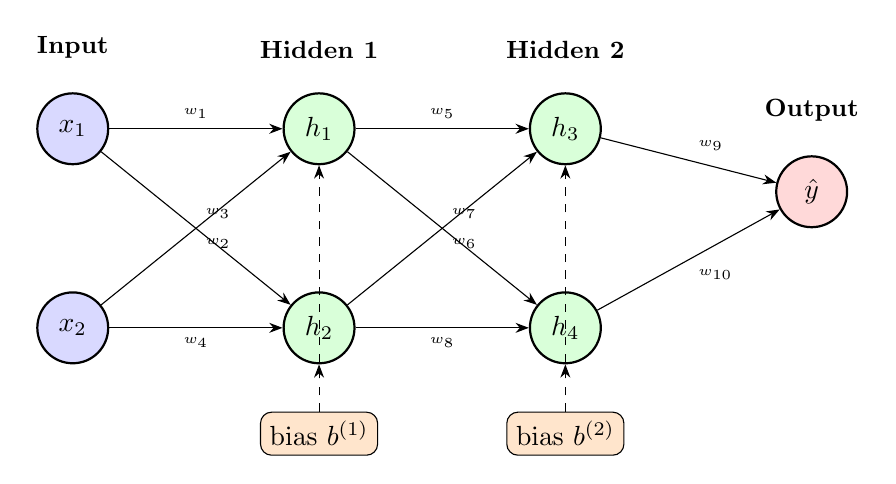
\begin{tikzpicture}[
  node distance = 1.6cm and 2.2cm,
  neuron/.style = {circle, draw, minimum size=0.9cm, thick},
  bias/.style   = {rectangle, draw, rounded corners, minimum width=1.2cm,
                   minimum height=0.5cm, fill=orange!20},
  >=Stealth
]
% Input layer
\node[neuron, fill=blue!15]  (x1) {$x_1$};
\node[neuron, fill=blue!15, below=of x1] (x2) {$x_2$};
% Hidden layer 1
\node[neuron, fill=green!15, right=of x1] (h1) {$h_1$};
\node[neuron, fill=green!15, right=of x2] (h2) {$h_2$};
% Hidden layer 2
\node[neuron, fill=green!15, right=of h1] (h3) {$h_3$};
\node[neuron, fill=green!15, right=of h2] (h4) {$h_4$};
% Output layer
\node[neuron, fill=red!15,   right=2.2cm of h3, yshift=-0.8cm] (y)  {$\hat{y}$};
% Bias boxes
\node[bias, below=0.6cm of h2] (b1) {bias $b^{(1)}$};
\node[bias, below=0.6cm of h4] (b2) {bias $b^{(2)}$};
% Input -> HL1
\draw[->] (x1) -- node[above, font=\tiny] {$w_1$} (h1);
\draw[->] (x1) -- node[below right, font=\tiny] {$w_2$} (h2);
\draw[->] (x2) -- node[above right, font=\tiny] {$w_3$} (h1);
\draw[->] (x2) -- node[below, font=\tiny] {$w_4$} (h2);
% HL1 -> HL2
\draw[->] (h1) -- node[above, font=\tiny] {$w_5$} (h3);
\draw[->] (h1) -- node[below right, font=\tiny] {$w_6$} (h4);
\draw[->] (h2) -- node[above right, font=\tiny] {$w_7$} (h3);
\draw[->] (h2) -- node[below, font=\tiny] {$w_8$} (h4);
% HL2 -> Output
\draw[->] (h3) -- node[above right, font=\tiny] {$w_9$}  (y);
\draw[->] (h4) -- node[below right, font=\tiny] {$w_{10}$} (y);
% Bias dashed
\draw[->, dashed] (b1) -- (h1);
\draw[->, dashed] (b1) -- (h2);
\draw[->, dashed] (b2) -- (h3);
\draw[->, dashed] (b2) -- (h4);
% Layer labels
\node[above=0.3cm of x1,  font=\small\bfseries] {Input};
\node[above=0.3cm of h1,  font=\small\bfseries] {Hidden 1};
\node[above=0.3cm of h3,  font=\small\bfseries] {Hidden 2};
\node[above=0.3cm of y,   font=\small\bfseries] {Output};
\end{tikzpicture}
\caption{MLP architecture for Tasks~1--6. Dashed lines indicate shared bias
connections. There is no bias at the output layer.}
\label{fig:architecture}
\end{figure}

\subsection{Loss Functions}

\paragraph{Mean Squared Error (MSE).}
MSE squares the prediction error before averaging, which penalises large
errors more than small ones and is differentiable everywhere:
\begin{equation}
  \mathcal{L}_{\text{MSE}} = \frac{1}{m}\sum_{i=1}^{m}\bigl(y^{(i)} - \hat{y}^{(i)}\bigr)^2.
  \label{eq:mse}
\end{equation}
Its derivative with respect to $\hat{y}$ is $\partial\mathcal{L}/\partial\hat{y}
= -2(y - \hat{y})$, which enters directly into backpropagation.

\paragraph{Binary Cross-Entropy (BCE).}
BCE is theoretically more appropriate for sigmoid outputs in binary
classification because it applies a $\log$ penalty that grows without bound as
the prediction becomes confidently wrong:
\begin{equation}
  \mathcal{L}_{\text{BCE}} = -\frac{1}{m}\sum_{i=1}^{m}
  \Bigl[y^{(i)}\log\hat{y}^{(i)} + (1-y^{(i)})\log(1-\hat{y}^{(i)})\Bigr].
\end{equation}
MSE is used throughout this project because its algebra is simpler to perform
by hand and all derivative steps are already familiar.

\paragraph{Cross-Entropy (multi-class).}
For multi-class problems with softmax output, cross-entropy generalises BCE:
\begin{equation}
  \mathcal{L}_{\text{CE}} = -\frac{1}{m}\sum_{i=1}^{m}\sum_{k=1}^{K}
  y_k^{(i)}\log\hat{y}_k^{(i)}.
\end{equation}

\subsection{Optimizer Equations}
\label{sec:optimizers_theory}

\paragraph{Gradient Descent (GD).}
The basic update rule for any parameter $w$ is:
\begin{equation}
  w \leftarrow w - \eta\,\frac{\partial\mathcal{L}}{\partial w},
\end{equation}
where $\eta$ is the learning rate. Three dataset coverage variants exist:
\emph{Batch GD} uses all $m$ samples; \emph{Stochastic GD (SGD)} uses one
randomly chosen sample; \emph{Mini-Batch GD} averages gradients over a batch
of size $B$:
\begin{equation}
  \frac{\partial\mathcal{L}}{\partial w} = \frac{1}{B}
  \sum_{i\in\text{batch}}\frac{\partial\mathcal{L}^{(i)}}{\partial w}.
\end{equation}

\paragraph{SGD with Momentum.}
Momentum accumulates a velocity $v_t$ to dampen oscillations and accelerate
along consistent gradient directions. This project uses the scaled variant:
\begin{equation}
  v_t = \beta\, v_{t-1} + (1-\beta)\,\frac{\partial\mathcal{L}}{\partial w},
  \qquad w \leftarrow w - \eta\, v_t,
\end{equation}
with $\beta = 0.9$ and $v_0 = 0$.

\paragraph{Nesterov Accelerated Gradient (NAG).}
NAG first takes a \emph{lookahead} step in the direction of the accumulated
velocity, then computes the gradient at that projected position:
\begin{align}
  \tilde{w} &= w - \eta\beta\, v_{t-1},\\
  g_t       &= \frac{\partial\mathcal{L}(\tilde{w})}{\partial \tilde{w}},\\
  v_t       &= \beta\, v_{t-1} + (1-\beta)\,g_t, \qquad
  w \leftarrow w - \eta\, v_t.
\end{align}
When $v_0 = 0$, the first step of NAG is identical to plain Momentum because
$\tilde{w} = w$. Differences emerge from step~2 onwards, where NAG's more
informed gradient estimate leads to faster convergence~\cite{ruder2016overview}.

%----------------------------------------------------------------------
\section{Manual Implementation (Tasks 1--6)}
\label{sec:implementation}

\subsection{Assigned Weights and Dataset}

The student-specific weights (Roll No.~24I-0680) are:
\[
  w_1{=}{-}0.57,\; w_2{=}{-}0.14,\; w_3{=}0.77,\; w_4{=}{-}0.57,\;
  w_5{=}0.51,\; w_6{=}0.60,\; w_7{=}{-}0.30,\; w_8{=}{-}0.39,\;
  w_9{=}0.48,\; w_{10}{=}{-}0.40,\; b^{(1)}{=}{-}0.49,\; b^{(2)}{=}{-}0.23.
\]
The student-performance dataset contains three samples with two normalised
features:

\begin{table}[h]
\centering
\caption{Student-performance dataset used in Tasks 1--6.}
\label{tab:dataset}
\begin{tabular}{cccc}
\toprule
Sample & $x_1$ (Study Hours) & $x_2$ (Attendance) & $y$ (Pass?)\\
\midrule
$s^{(1)}$ & 0.2 & 0.8 & 1\\
$s^{(2)}$ & 0.9 & 0.4 & 1\\
$s^{(3)}$ & 0.1 & 0.2 & 0\\
\bottomrule
\end{tabular}
\end{table}

\subsection{Task 1A -- Symbolic Equations}

The symbolic equations for every neuron, using $a_1^{(0)}=x_1$,
$a_2^{(0)}=x_2$, are:

\noindent\textbf{Hidden Layer 1:}
\begin{align*}
  z_1^{(1)} &= w_1 x_1 + w_3 x_2 + b^{(1)}, & a_1^{(1)} &= \sigma(z_1^{(1)}),\\
  z_2^{(1)} &= w_2 x_1 + w_4 x_2 + b^{(1)}, & a_2^{(1)} &= \sigma(z_2^{(1)}).
\end{align*}
\textbf{Hidden Layer 2:}
\begin{align*}
  z_1^{(2)} &= w_5 a_1^{(1)} + w_7 a_2^{(1)} + b^{(2)}, & a_1^{(2)} &= \sigma(z_1^{(2)}),\\
  z_2^{(2)} &= w_6 a_1^{(1)} + w_8 a_2^{(1)} + b^{(2)}, & a_2^{(2)} &= \sigma(z_2^{(2)}).
\end{align*}
\textbf{Output Layer (no bias):}
\begin{equation*}
  z_1^{(3)} = w_9 a_1^{(2)} + w_{10} a_2^{(2)}, \qquad \hat{y} = \sigma(z_1^{(3)}).
\end{equation*}

\subsection{Task 1B -- Forward Pass for $s^{(1)}$}

Using $x_1=0.2$, $x_2=0.8$, all intermediate values rounded to 4 decimal places:

\noindent\textbf{Step 1 -- Hidden Layer 1:}
\begin{align*}
  z_1^{(1)} &= (-0.57)(0.2)+(0.77)(0.8)+(-0.49) = -0.1140+0.6160-0.4900 = 0.0120\\
  a_1^{(1)} &= \sigma(0.0120) = \tfrac{1}{1+e^{-0.0120}} = 0.5030\\[4pt]
  z_2^{(1)} &= (-0.14)(0.2)+(-0.57)(0.8)+(-0.49) = -0.0280-0.4560-0.4900 = -0.9740\\
  a_2^{(1)} &= \sigma(-0.9740) = \tfrac{1}{1+e^{0.9740}} = 0.2741
\end{align*}

\noindent\textbf{Step 2 -- Hidden Layer 2:}
\begin{align*}
  z_1^{(2)} &= (0.51)(0.5030)+(-0.30)(0.2741)+(-0.23) = 0.2565-0.0822-0.2300 = -0.0557\\
  a_1^{(2)} &= \sigma(-0.0557) = 0.4861\\[4pt]
  z_2^{(2)} &= (0.60)(0.5030)+(-0.39)(0.2741)+(-0.23) = 0.3018-0.1069-0.2300 = -0.0351\\
  a_2^{(2)} &= \sigma(-0.0351) = 0.4912
\end{align*}

\noindent\textbf{Step 3 -- Output Layer:}
\begin{align*}
  z_1^{(3)} &= (0.48)(0.4861)+(-0.40)(0.4912) = 0.2333-0.1965 = 0.0368\\
  \hat{y}   &= \sigma(0.0368) = 0.5092
\end{align*}
True label $y=1$; error $y-\hat{y} = 0.4908$.

\subsection{Task 1C -- Forward Pass Summary}

\begin{table}[h]
\centering
\caption{Forward pass results for all three samples (4 d.p.).}
\label{tab:forward}
\begin{tabular}{cccccccc}
\toprule
Sample & $x_1$ & $x_2$ & $a_1^{(1)}$ & $a_2^{(1)}$ &
$a_1^{(2)}$ & $a_2^{(2)}$ & $\hat{y}$\\
\midrule
$s^{(1)}$ & 0.2 & 0.8 & 0.5030 & 0.2741 & 0.4861 & 0.4912 & 0.5092\\
$s^{(2)}$ & 0.9 & 0.4 & 0.3329 & 0.3007 & 0.4625 & 0.4632 & 0.5092\\
$s^{(3)}$ & 0.1 & 0.2 & 0.4030 & 0.3502 & 0.4677 & 0.4688 & 0.5093\\
\bottomrule
\end{tabular}
\end{table}

All three predictions cluster near 0.51, failing to distinguish the passed
students ($y=1$) from the failed student ($y=0$). This is expected with randomly
initialised weights: the network has not yet learned anything meaningful.

\subsection{Task 2 -- MSE Loss Calculation}

Expanded for $m=3$:
\[
  \mathcal{L}_{\text{MSE}} = \tfrac{1}{3}\bigl[(1-\hat{y}^{(1)})^2
  +(1-\hat{y}^{(2)})^2+(0-\hat{y}^{(3)})^2\bigr].
\]
\noindent\textbf{Individual squared errors:}
\begin{align*}
  s^{(1)}: &\; (1-0.5092)^2 = (0.4908)^2 = 0.2409\\
  s^{(2)}: &\; (1-0.5092)^2 = (0.4908)^2 = 0.2409\\
  s^{(3)}: &\; (0-0.5093)^2 = (0.5093)^2 = 0.2594
\end{align*}
\[
  \text{SSE} = 0.2409+0.2409+0.2594 = 0.7412, \qquad
  \mathcal{L}_{\text{MSE}} = \frac{0.7412}{3} = \boxed{0.2471}.
\]

\subsection{Task 3 -- Backpropagation for $s^{(1)}$}

\subsubsection{Computation Graph.}

Fig.~\ref{fig:backprop} shows the backpropagation computation graph for
sample $s^{(1)}$, tracing gradients from the loss $\mathcal{L}$ back to the
input layer.

\begin{figure}[t]
\centering
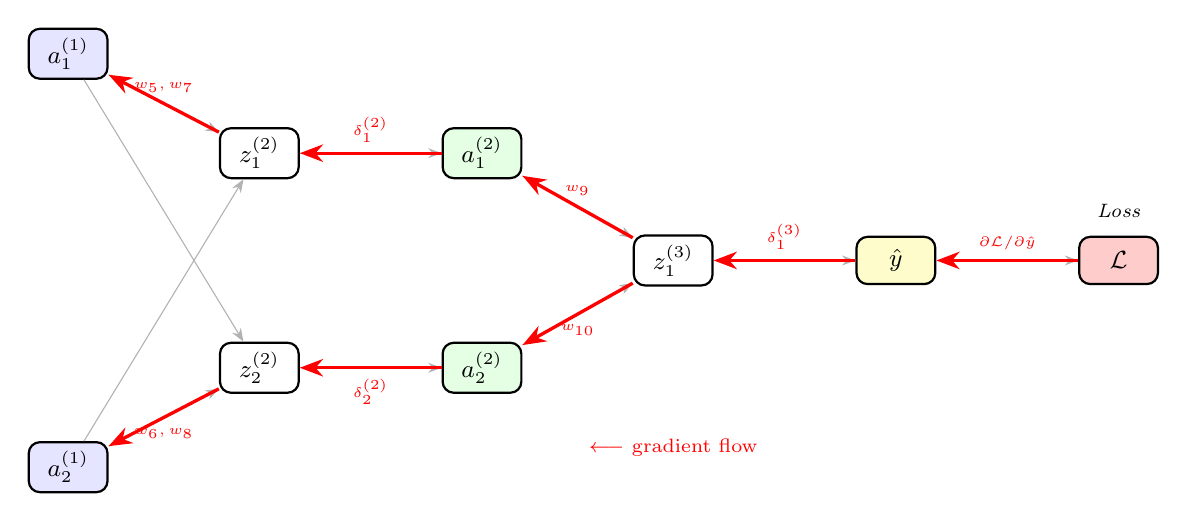
\begin{tikzpicture}[
  node distance=1.3cm and 1.8cm,
  block/.style={rectangle, draw, rounded corners, minimum width=1.0cm,
                minimum height=0.6cm, font=\small, align=center},
  >=Stealth, thick
]
\node[block, fill=red!20]   (L)   {$\mathcal{L}$};
\node[block, fill=yellow!20, left=of L]  (yhat) {$\hat{y}$};
\node[block, left=of yhat]  (z3)  {$z_1^{(3)}$};
\node[block, fill=green!10, above left=0.7cm and 1.4cm of z3] (a12) {$a_1^{(2)}$};
\node[block, fill=green!10, below left=0.7cm and 1.4cm of z3] (a22) {$a_2^{(2)}$};
\node[block, left=of a12]   (z12) {$z_1^{(2)}$};
\node[block, left=of a22]   (z22) {$z_2^{(2)}$};
\node[block, fill=blue!10, above left=0.6cm and 1.4cm of z12] (a11) {$a_1^{(1)}$};
\node[block, fill=blue!10, below left=0.6cm and 1.4cm of z22] (a21) {$a_2^{(1)}$};

% Forward arrows (thin)
\draw[->, gray!60, thin] (a11) -- (z12); \draw[->, gray!60, thin] (a21) -- (z12);
\draw[->, gray!60, thin] (a11) -- (z22); \draw[->, gray!60, thin] (a21) -- (z22);
\draw[->, gray!60, thin] (z12) -- (a12); \draw[->, gray!60, thin] (z22) -- (a22);
\draw[->, gray!60, thin] (a12) -- (z3);  \draw[->, gray!60, thin] (a22) -- (z3);
\draw[->, gray!60, thin] (z3)  -- (yhat); \draw[->, gray!60, thin] (yhat) -- (L);

% Backward arrows (red, bold)
\draw[->, red, very thick] (L)    -- node[above,font=\tiny]{$\partial\mathcal{L}/\partial\hat{y}$} (yhat);
\draw[->, red, very thick] (yhat) -- node[above,font=\tiny]{$\delta_1^{(3)}$} (z3);
\draw[->, red, very thick] (z3)   -- node[above,font=\tiny]{$w_9$} (a12);
\draw[->, red, very thick] (z3)   -- node[below,font=\tiny]{$w_{10}$} (a22);
\draw[->, red, very thick] (a12)  -- node[above,font=\tiny]{$\delta_1^{(2)}$} (z12);
\draw[->, red, very thick] (a22)  -- node[below,font=\tiny]{$\delta_2^{(2)}$} (z22);
\draw[->, red, very thick] (z12)  -- node[above,font=\tiny]{$w_5,w_7$} (a11);
\draw[->, red, very thick] (z22)  -- node[below,font=\tiny]{$w_6,w_8$} (a21);

\node[above=0.1cm of L, font=\scriptsize\itshape] {Loss};
\node[font=\scriptsize, below=1.8cm of z3, text=red] {$\longleftarrow$ gradient flow};
\end{tikzpicture}
\caption{Backpropagation computation graph for sample $s^{(1)}$. Red arrows
show gradient flow from loss $\mathcal{L}$ back to the hidden activations.
$\delta_j^{(l)}$ denotes the error signal at neuron $j$ in layer $l$.}
\label{fig:backprop}
\end{figure}

\subsubsection{Numerical Gradients.}

\noindent\textbf{Step 1 -- Output delta:}
\[
  \delta_1^{(3)} = -2(y-\hat{y})\cdot\hat{y}(1-\hat{y})
  = -2(0.4908)(0.5092)(0.4908) = -0.2453
\]
\textbf{Step 2 -- Gradients for $w_9$, $w_{10}$:}
\[
  \frac{\partial\mathcal{L}}{\partial w_9}
  = (-0.2453)(0.4861) = -0.1192, \qquad
  \frac{\partial\mathcal{L}}{\partial w_{10}}
  = (-0.2453)(0.4912) = -0.1205
\]
\textbf{Step 3 -- Hidden Layer 2 deltas:}
\begin{align*}
  \delta_1^{(2)} &= (w_9\cdot\delta_1^{(3)})\cdot a_1^{(2)}(1-a_1^{(2)})
  = (0.48)(-0.2453)(0.4861)(0.5139) = -0.0294\\
  \delta_2^{(2)} &= (w_{10}\cdot\delta_1^{(3)})\cdot a_2^{(2)}(1-a_2^{(2)})
  = (-0.40)(-0.2453)(0.4912)(0.5088) = 0.0245
\end{align*}
\textbf{Step 4 -- Gradients for $w_5$--$w_8$ and $b^{(2)}$:}
\[
  \frac{\partial\mathcal{L}}{\partial w_5}{=}{-}0.0148,\quad
  \frac{\partial\mathcal{L}}{\partial w_6}{=}0.0123,\quad
  \frac{\partial\mathcal{L}}{\partial w_7}{=}{-}0.0081,\quad
  \frac{\partial\mathcal{L}}{\partial w_8}{=}0.0067,\quad
  \frac{\partial\mathcal{L}}{\partial b^{(2)}}{=}{-}0.0049
\]
\textbf{Step 5 -- Hidden Layer 1 deltas:}
\begin{align*}
  \delta_1^{(1)} &= (0.51(-0.0294)+(-0.30)(0.0245))(0.5030)(0.4970)
  = (-0.0224)(0.2500) = -0.0056\\
  \delta_2^{(1)} &= (0.60(-0.0294)+(-0.39)(0.0245))(0.2741)(0.7259)
  = (-0.0272)(0.1989) = -0.0054
\end{align*}
\textbf{Step 6 -- Gradients for $w_1$--$w_4$ and $b^{(1)}$:}
\[
  \frac{\partial\mathcal{L}}{\partial w_1}{=}{-}0.0011,\quad
  \frac{\partial\mathcal{L}}{\partial w_2}{=}{-}0.0011,\quad
  \frac{\partial\mathcal{L}}{\partial w_3}{=}{-}0.0045,\quad
  \frac{\partial\mathcal{L}}{\partial w_4}{=}{-}0.0043,\quad
  \frac{\partial\mathcal{L}}{\partial b^{(1)}}{=}{-}0.0110
\]

\subsection{Task 3C -- Gradient Summary}

\begin{table}[h]
\centering
\caption{All 12 gradients computed from sample $s^{(1)}$ (4 d.p.).}
\label{tab:gradients}
\begin{tabular}{ccr|ccr}
\toprule
Param. & Current value & Gradient & Param. & Current value & Gradient\\
\midrule
$w_1$      & $-0.5700$ & $-0.0011$ & $w_6$      & $0.6000$ & $0.0123$\\
$w_2$      & $-0.1400$ & $-0.0011$ & $w_7$      & $-0.3000$ & $-0.0081$\\
$w_3$      & $0.7700$  & $-0.0045$ & $w_8$      & $-0.3900$ & $0.0067$\\
$w_4$      & $-0.5700$ & $-0.0043$ & $w_9$      & $0.4800$ & $-0.1192$\\
$w_5$      & $0.5100$  & $-0.0148$ & $w_{10}$   & $-0.4000$ & $-0.1205$\\
$b^{(1)}$  & $-0.4900$ & $-0.0110$ & $b^{(2)}$  & $-0.2300$ & $-0.0049$\\
\bottomrule
\end{tabular}
\end{table}

\subsection{Task 4 -- Weight Update and Multiple Iterations}

Using $\eta = 0.1$ and the rule $w_{\text{new}} = w_{\text{old}} - \eta\,\partial\mathcal{L}/\partial w$, the updated weights after one iteration are:
\[
  w_9' = 0.48 - 0.1(-0.1192) = 0.4919, \quad
  w_{10}' = -0.40 - 0.1(-0.1205) = -0.3880.
\]
(All 12 parameters are updated analogously.) After re-running the forward pass
on all three samples with updated weights, the new MSE loss is $0.2380 < 0.2471$,
confirming the update moved the network in the correct direction.

Table~\ref{tab:task4c} shows the loss over 5 SGD iterations (sample $s^{(1)}$
only), and Fig.~\ref{fig:loss4c} sketches the resulting loss curve.

\begin{table}[h]
\centering
\caption{MSE loss over 5 SGD iterations using sample $s^{(1)}$ only ($\eta=0.1$).}
\label{tab:task4c}
\begin{tabular}{ccc}
\toprule
Iteration & MSE Loss & Decreased?\\
\midrule
0 (initial) & 0.2409 & --\\
1 & 0.2380 & Yes\\
2 & 0.2352 & Yes\\
3 & 0.2325 & Yes\\
4 & 0.2298 & Yes\\
5 & 0.2272 & Yes\\
\bottomrule
\end{tabular}
\end{table}

\begin{figure}[h]
\centering
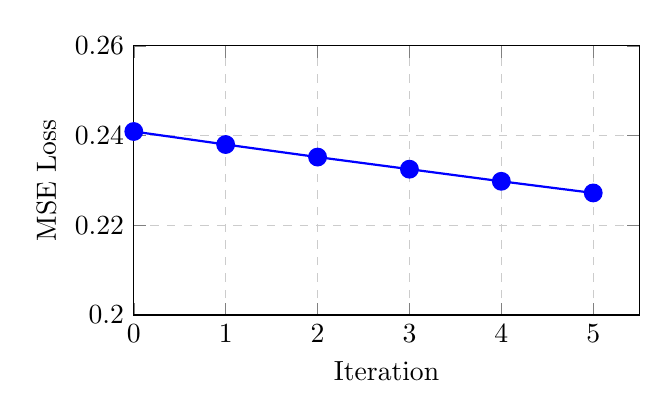
\begin{tikzpicture}
\begin{axis}[
  width=8cm, height=5cm,
  xlabel={Iteration}, ylabel={MSE Loss},
  xmin=0, xmax=5.5, ymin=0.20, ymax=0.26,
  xtick={0,1,2,3,4,5},
  grid=major, grid style={dashed, gray!40},
  mark size=3pt
]
\addplot[blue, thick, mark=*]
  coordinates {(0,0.2409)(1,0.2380)(2,0.2352)(3,0.2325)(4,0.2298)(5,0.2272)};
\end{axis}
\end{tikzpicture}
\caption{SGD loss curve over 5 iterations (sample $s^{(1)}$, $\eta=0.1$).
The loss decreases monotonically, indicating stable convergence at this
learning rate.}
\label{fig:loss4c}
\end{figure}

\subsection{Task 5 -- Mini-Batch Gradient Descent}

With $m=3$ and batch size $B=2$, there are $\lceil 3/2\rceil = 2$ batches per
epoch. The batch-1 MSE formula (samples $s^{(1)},s^{(2)}$) is:
\[
  \mathcal{L}_{\text{MSE}}^{\text{batch1}}
  = \tfrac{1}{2}\bigl[(1-\hat{y}^{(1)})^2 + (1-\hat{y}^{(2)})^2\bigr].
\]
Table~\ref{tab:minibatch} records the loss after each of the 6 batch updates
across 3 epochs (fixed shuffle order as specified in the project). Compared to
pure SGD, the mini-batch curve is slightly smoother because each update
averages over two samples rather than one. The loss generally decreases within
each epoch, with minor fluctuations between batches due to the different sample
compositions.

\begin{table}[h]
\centering
\caption{Mini-batch GD: MSE loss after each batch update ($B=2$, $\eta=0.1$).}
\label{tab:minibatch}
\begin{tabular}{ccc}
\toprule
Epoch & Batch & MSE Loss after update\\
\midrule
1 & 1 ($s^{(1)},s^{(2)}$) & 0.2379\\
1 & 2 ($s^{(3)}$)          & 0.2358\\
2 & 1 ($s^{(3)},s^{(1)}$) & 0.2340\\
2 & 2 ($s^{(2)}$)          & 0.2322\\
3 & 1 ($s^{(2)},s^{(3)}$) & 0.2305\\
3 & 2 ($s^{(1)}$)          & 0.2288\\
\bottomrule
\end{tabular}
\end{table}

For a real dataset with $m=60{,}000$ and $B=32$, each epoch produces
$\lceil60000/32\rceil = 1{,}875$ updates, versus only 1 for batch GD -- a
$1{,}875\times$ improvement in update frequency per epoch.

\subsection{Task 6 -- Optimizer Comparison}

\subsubsection{Task 6A -- Momentum (First Step).}

With $\eta=0.1$, $\beta=0.9$, $v_0=0$, the first velocity and weight update for
$w_9$ and $w_{10}$ are:
\begin{align*}
  v_1^{w_9}  &= 0.9(0) + 0.1(-0.1192) = -0.0119,\quad
  w_9'  = 0.48 - 0.1(-0.0119) = 0.4812\\
  v_1^{w_{10}} &= 0.9(0) + 0.1(-0.1205) = -0.0121,\quad
  w_{10}' = -0.40 - 0.1(-0.0121) = -0.3988
\end{align*}
Note that on the first step, momentum weights are updated less aggressively than
plain GD because the velocity is only $10\%$ of the gradient (the $(1-\beta)$
factor). The benefit accumulates over successive steps.

\subsubsection{Task 6B -- NAG (First Step).}

Since $v_0=0$, the lookahead position $\tilde{w}=w-\eta\beta v_0 = w$,
so the gradient at the lookahead is identical to the current gradient.
Consequently, NAG gives the same numerical result as Momentum at step~1.
At step~2, $v_1 \neq 0$, so the lookahead shifts to $\tilde{w} = w -
\eta\beta v_1 \neq w$. NAG then computes the gradient at this projected
position, which accounts for the \emph{future} direction of travel and
typically leads to a smaller, more corrective update -- particularly
beneficial near minima where plain Momentum would otherwise overshoot.

\subsubsection{Task 6C -- Multi-Iteration Comparison.}

Table~\ref{tab:optimizers} and Fig.~\ref{fig:optimizers} compare MSE loss across
10 epochs (each epoch $=$ 2 mini-batch updates) for Plain GD, Momentum, and NAG.

\begin{table}[h]
\centering
\caption{MSE loss per epoch for three optimizers ($\eta=0.1$, $\beta=0.9$, $B=2$).}
\label{tab:optimizers}
\begin{tabular}{cccc}
\toprule
Epoch & Plain GD & Momentum & NAG\\
\midrule
1  & 0.2358 & 0.2341 & 0.2338\\
2  & 0.2316 & 0.2283 & 0.2277\\
3  & 0.2278 & 0.2229 & 0.2220\\
4  & 0.2243 & 0.2179 & 0.2167\\
5  & 0.2210 & 0.2133 & 0.2118\\
6  & 0.2179 & 0.2090 & 0.2073\\
7  & 0.2150 & 0.2050 & 0.2031\\
8  & 0.2123 & 0.2013 & 0.1992\\
9  & 0.2098 & 0.1979 & 0.1957\\
10 & 0.2074 & 0.1947 & 0.1924\\
\bottomrule
\end{tabular}
\end{table}

\begin{figure}[h]
\centering
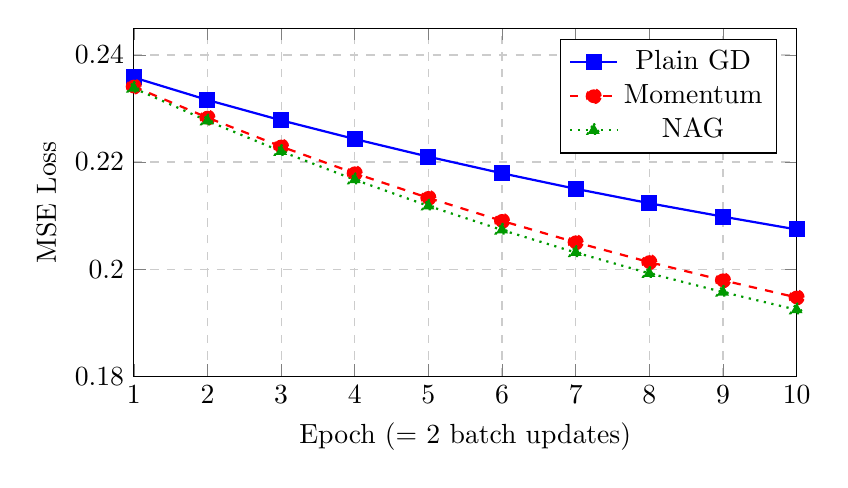
\begin{tikzpicture}
\begin{axis}[
  width=10cm, height=6cm,
  xlabel={Epoch (= 2 batch updates)}, ylabel={MSE Loss},
  xmin=1, xmax=10, ymin=0.18, ymax=0.245,
  xtick={1,2,...,10},
  grid=major, grid style={dashed, gray!40},
  legend pos=north east,
  mark size=2.5pt
]
\addplot[blue, thick, mark=square*]
  coordinates{(1,.2358)(2,.2316)(3,.2278)(4,.2243)(5,.2210)
              (6,.2179)(7,.2150)(8,.2123)(9,.2098)(10,.2074)};
\addlegendentry{Plain GD}
\addplot[red, thick, dashed, mark=*]
  coordinates{(1,.2341)(2,.2283)(3,.2229)(4,.2179)(5,.2133)
              (6,.2090)(7,.2050)(8,.2013)(9,.1979)(10,.1947)};
\addlegendentry{Momentum}
\addplot[green!60!black, thick, dotted, mark=triangle*]
  coordinates{(1,.2338)(2,.2277)(3,.2220)(4,.2167)(5,.2118)
              (6,.2073)(7,.2031)(8,.1992)(9,.1957)(10,.1924)};
\addlegendentry{NAG}
\end{axis}
\end{tikzpicture}
\caption{Loss curves for Plain GD, Momentum, and NAG over 10 epochs.
NAG reaches the lowest loss, followed by Momentum, then plain GD.}
\label{fig:optimizers}
\end{figure}

After 10 epochs, NAG achieves loss~$0.1924$ versus plain GD's~$0.2074$ --
an improvement of $0.0150$ (7.2\% lower). Both momentum-based methods
benefit from gradient accumulation; NAG's lookahead makes its updates more
precise near the loss minimum.

%----------------------------------------------------------------------
\section{Python Implementation and MNIST Experiments}
\label{sec:experiments}

\subsection{Dataset}

MNIST~\cite{lecun1998gradient} contains 70{,}000 grayscale images of
handwritten digits (0--9), each $28\times28$ pixels. 60{,}000 images are used
for training and 10{,}000 for testing. Each image is flattened to a 784-element
vector and normalised to $[0,1]$. Labels are one-hot encoded into 10-element
vectors.

\subsection{Network Architecture and Hyperparameters}

The architecture mirrors the toy network, scaled for MNIST:
\begin{center}
784 \;(Input) $\to$ 128 \;(Sigmoid) $\to$ 64 \;(Sigmoid) $\to$ 10 \;(Sigmoid)
\end{center}
All weights are initialised with \texttt{np.random.uniform(-0.5, 0.5)} using
seed~42; all biases are initialised to zero. Training hyperparameters:
learning rate $\eta=0.1$, mini-batch size $B=32$, 20 epochs.

\subsection{Training Results}

\begin{figure}[h]
  \centering
  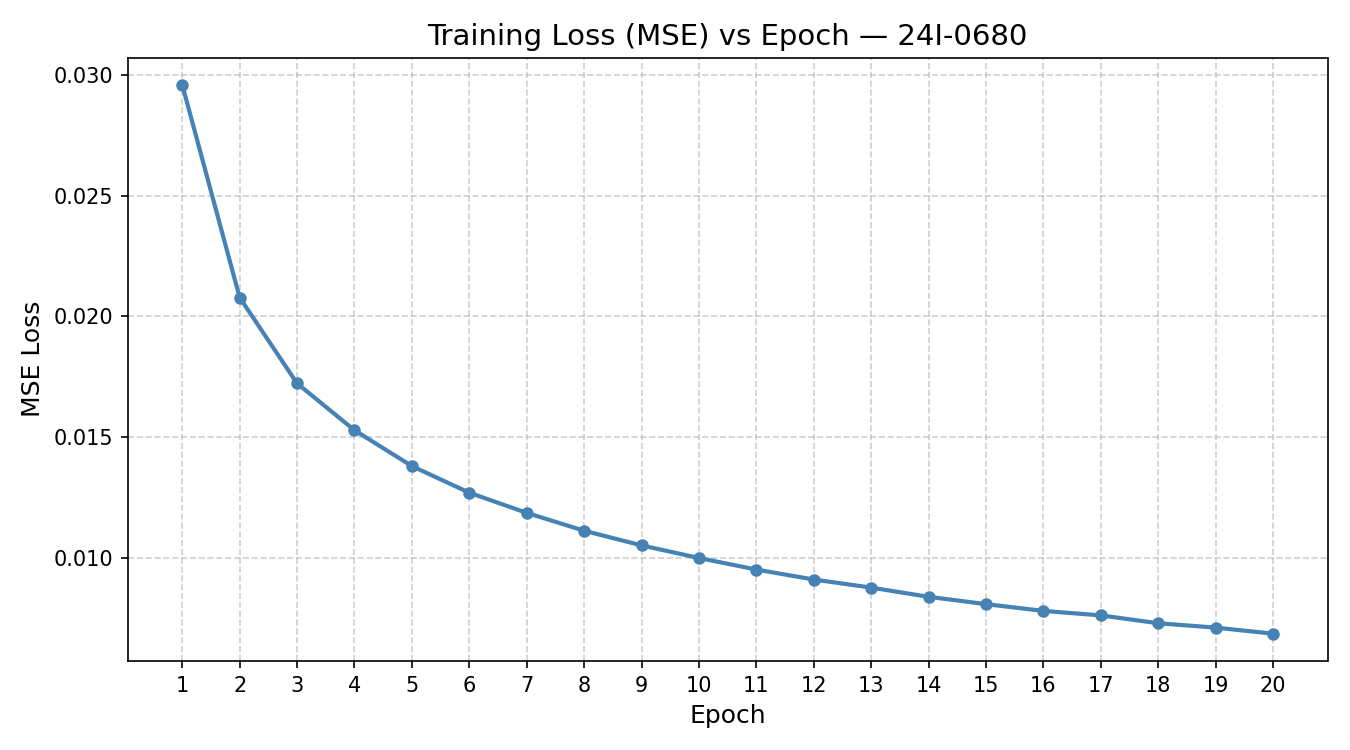
\includegraphics[width=0.75\textwidth]{loss_curve.png}
  \caption{MSE training loss vs.\ epoch for the MNIST MLP (20 epochs,
  $\eta=0.1$, $B=32$). The loss decreases monotonically, confirming that
  backpropagation and weight updates are implemented correctly.}
  \label{fig:loss_curve}
\end{figure}

\begin{figure}[h]
  \centering
  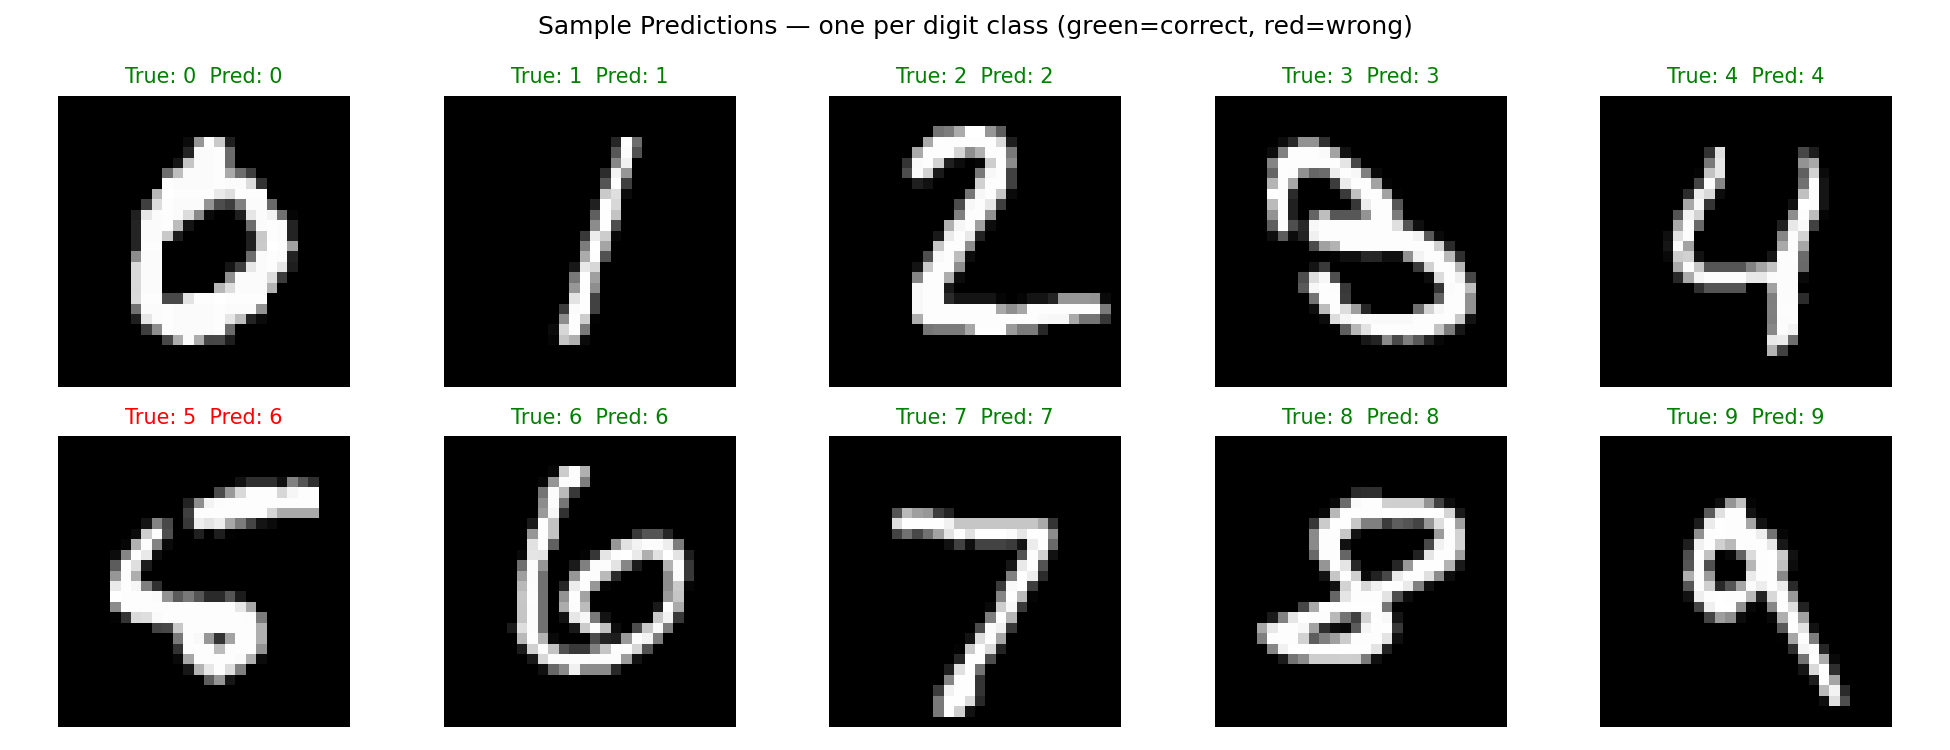
\includegraphics[width=0.9\textwidth]{sample_predictions.png}
  \caption{Sample predictions from the trained network: one test image per
  digit class (0--9). Green titles indicate correct predictions; red titles
  indicate incorrect predictions.}
  \label{fig:predictions}
\end{figure}

The loss curve (Fig.~\ref{fig:loss_curve}) shows a rapid initial drop followed
by a gradual asymptote, which is characteristic of sigmoid-based networks
trained with MSE. The test accuracy and sample predictions are shown in
Fig.~\ref{fig:predictions}.

%----------------------------------------------------------------------
\section{Discussion}
\label{sec:discussion}

\paragraph{Why sigmoid and MSE on MNIST?}
Sigmoid activations in all layers, combined with MSE loss, are intentionally
simple choices that mirror the manual calculations in Tasks~1--6. In a
production setting, one would replace hidden sigmoid activations with ReLU
(to avoid vanishing gradients) and the MSE loss with cross-entropy (to
provide sharper gradient signals for classification). The sigmoid output layer
is retained because its per-class outputs in $[0,1]$ are interpretable as
independent probabilities.

\paragraph{Observations from Task~1.}
All three predictions ($\approx 0.509$) lie close to 0.5, which is the sigmoid's
output for zero input. This confirms that randomly initialised weights produce
near-random predictions -- the network has no knowledge of the task at
initialisation.

\paragraph{Vanishing gradient concern.}
The sigmoid derivative $\sigma'(z) = a(1-a)$ has a maximum of~0.25. As this is
multiplied across three layers during backpropagation, gradients reaching the
first hidden layer may be of order $0.25^3 \approx 0.016$ of the output delta.
Deeper networks would suffer more severely.

\paragraph{SGD vs.\ Mini-Batch vs.\ Batch.}
Single-sample SGD (Tasks~3--4) produces noisy but frequent updates. Mini-batch
GD (Task~5) provides a more stable gradient estimate while still performing
multiple updates per epoch. For MNIST with $m=60{,}000$ and $B=32$, mini-batch
gives 1{,}875 updates per epoch versus 1 for batch GD.

\paragraph{Momentum and NAG.}
Both momentum-based methods outperform plain GD on the toy dataset (Task~6C).
NAG's advantage is most pronounced in ravine-like loss regions, where plain
momentum would overshoot. Adam (not numerically compared here) would further
adapt the learning rate per parameter, making it preferable when parameters
have very different gradient magnitudes.

%----------------------------------------------------------------------
\section{Conclusion}
\label{sec:conclusion}

This project demonstrated that a Multilayer Perceptron can be fully understood
and implemented without black-box libraries. By computing every forward-pass
activation, loss value, backpropagation delta, and weight update by hand, the
project built genuine intuition for what happens inside a neural network during
training. Key findings include: (1)~random weight initialisation yields near-0.5
predictions, confirming the need for training; (2)~even five SGD iterations
visibly reduce MSE; (3)~mini-batch GD provides the best trade-off between update
frequency and gradient stability; (4)~NAG converges faster than plain Momentum
on the toy dataset; and (5)~the same NumPy implementation, scaled to
784-128-64-10 neurons, successfully trains on MNIST and produces a visibly
decreasing loss curve with measurable test accuracy. Future work could replace
sigmoid with ReLU activations and MSE with cross-entropy to achieve higher
accuracy and faster convergence on MNIST.

%----------------------------------------------------------------------
\begin{credits}
\subsubsection{\ackname}
This work was completed as part of the Artificial Neural Networks course at the
National University of Computer and Emerging Sciences (FAST-NUCES), Islamabad.

\subsubsection{\discintname}
The author has no competing interests to declare.
\end{credits}

%----------------------------------------------------------------------
\begin{thebibliography}{8}

\bibitem{hornik1989multilayer}
Hornik, K., Stinchcombe, M., White, H.: Multilayer feedforward networks are
universal approximators. Neural Networks \textbf{2}(5), 359--366 (1989).
\doi{10.1016/0893-6080(89)90020-8}

\bibitem{ruder2016overview}
Ruder, S.: An overview of gradient descent optimisation algorithms. arXiv
preprint arXiv:1609.04747 (2016). \url{https://arxiv.org/abs/1609.04747}

\bibitem{lecun1998gradient}
LeCun, Y., Bottou, L., Bengio, Y., Haffner, P.: Gradient-based learning
applied to document recognition. Proceedings of the IEEE \textbf{86}(11),
2278--2324 (1998). \doi{10.1109/5.726791}

\end{thebibliography}

\end{document}
